\section{Generalization and Regulation}
\textbf{In-sample error:} It is possible to find a model which perfectly fits the data (MSE = 0) This is the loss minimized
during the training phase, it is therefore also called \textbf{training error}.\\
$\rightarrow$ Our goal is to learn a model from data that generalizes well to new data. A good model has a low generalization error.\\
\textbf{Test Error (Generalization Error):} We get this by using two completely disjoint datasets: one to train the model and the other to calculate the classification error. Both datasets need to have values for y. The first dataset is called training data and the second, test data.

\subsection{Underfitting (High Bias)}
When we have the scenarion of underfitting we have choosen a too simple model. (in-sample error=Large, Generalization error=Larger)

\subsection{Overfitting (Low Bias)}
We have the scenarion of overfitting if we have choosen a too complex model (in-sample error=0, Generalization error=huge).

\subsection{Trainig-Set, Test-Set}
We cant calculate the generalization error! We can try to estimate the generalization error. We can split the data into a training-set and test-set (80/20). We fit the model to the training set and minimize the in-sample error. We evaluate the model with the test-set which estimates the generalization error.

\subsection{Bias Variance Tradeoff}
\begin{minipage}{0,5\linewidth}
	\textbf{Bias:} The inability for a ML method to capture the true relationsship (High match=low Bias, low match=high Bias)\\
	\textbf{Variance:} is the difference in fits between two data sets.
	Higher bias implies lower variance, lower bias implies higher variance
\end{minipage}
\begin{minipage}{0,5\linewidth}
	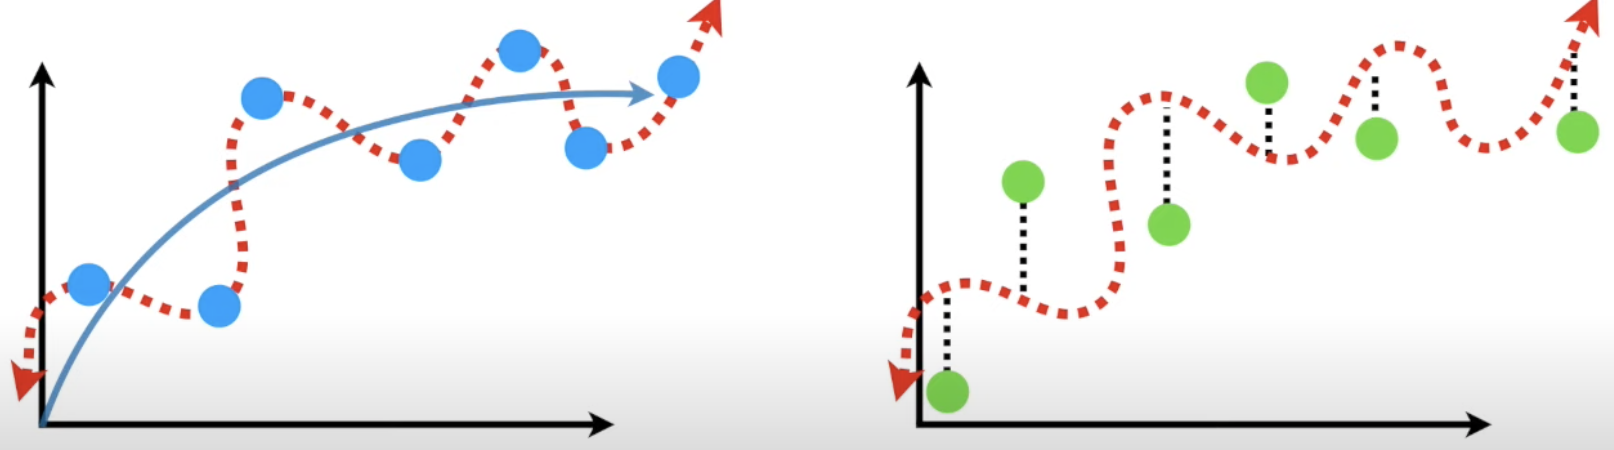
\includegraphics[width=0.9\linewidth]{biasvariance}\\
	Low Bias, High Variance
\end{minipage}
Note that we use the expression high bias in the sense of a too simple model for the given data and vica versa. High bias is a design by choice. $\rightarrow$ Find an optimal balance between bias and variance.

\subsection{Generalization}
We have to find the optimal balance between the variance and the bias with the help of generalization. We need to ingridient for regularization.
\begin{enumerate}[topsep=0pt]
  \itemsep -0.5em
  \item A Way to measure complexity: L1-Norm, L2-Norm
  \item A Way to control model complexity: penalty to loss, complex models get higher penalty.
\end{enumerate}

\subsection{Regularization}
Regularization is the most used technique to penalize complex models in machine learning, it is deployed for reducing overfitting by putting network weights small. Also, it enhances the performance of models for new inputs.

\subsubsection{L1-Norm (LASSO)}
It adds an L1 penalty that is equal to the absolute value of the magnitude of coefficient, or simply restricting the size of coefficients.
$\lambda$= Regularization Parameter (Hyper Par), $\beta$=Polynomial arguments. Lasso regression can do feature selection if a $\beta_{i}$=0.

\[ Cost = \frac{1}{2N} \sum_{i=1}^N (\hat{Y}-Y)^2 + \lambda \sum_{i=1}^N |\beta_{i}| \]

\subsubsection{L2-Norm (Ridge Regression)}
It adds an L2 penalty which is equal to the square of the magnitude of coefficients. $\beta_{0}$ is not regularized.

\[ Cost = \frac{1}{2N} \sum_{i=1}^N (\hat{Y}-Y)^2 + \lambda \sum_{i=1}^N \beta_{i}^2 \]


\subsubsection{L1 + L2 Norm (Elastic Net)}
Elastic net uses both the L2 and the L1 penalty. 


